\documentclass{article}

\usepackage{xr-hyper}
\usepackage{subfiles}
\usepackage{amsmath}
\usepackage[english]{babel}
\usepackage{graphicx}
\usepackage{float}
\usepackage[letterpaper,top=2cm,bottom=2cm,left=3cm,right=3cm,marginparwidth=1.75cm]{geometry}
\usepackage{parskip}
\usepackage{amsmath}
\usepackage{graphicx}
\usepackage[colorlinks=true, allcolors=black]{hyperref}
\usepackage{caption}
\usepackage{algorithm}
\usepackage[noend]{algpseudocode}
\usepackage{nicefrac}
\usepackage{bookmark}
\usepackage{titlesec}
\usepackage{tabularx}

\makeatletter
\def\BState{\State\hskip-\ALG@thistlm}
\makeatother

\algnewcommand{\IIf}[1]{\State\algorithmicif\ #1\ \algorithmicthen}
\algnewcommand{\EndIIf}{\unskip\ \algorithmicend\ \algorithmicif}
\algnewcommand{\LineComment}[1]{\State \(\triangleright\) #1}

\setcounter{secnumdepth}{4}
\titleformat{\paragraph}
{\normalfont\normalsize\itshape}{\theparagraph}{1em}{}
\titlespacing*{\paragraph}
{0pt}{3.25ex plus 1ex minus .2ex}{1.5ex plus .2ex}
\renewcommand{\arraystretch}{1.5}

% elsarticle-num
\bibliographystyle{elsarticle-num}
\graphicspath{ {./Images/} }
\captionsetup[figure]{font=small}
\title{Machine Learning in the calibration process of Discrete Particle Model: The case with Angle of Repose}
\author{Quang Hung Nguyen\\[1ex] \small Head Supervisor: Thomas Weinhart, Daily Supervisor: Anthony Thornton, Additional member: Chen Kuan. \\
\small Multi-Scale Mechanics Group, Faculty of Engineering Technology, University of Twente.} 
\date{}

\begin{document}
\maketitle

\begin{center}
    \Large\textbf{Abstract}
\end{center}


\begin{center}
    This research presents a comprehensive study on the use of machine learning in the calibration problem of the Discrete Particle Model, with a particular focus on one bulk parameter: the static angle of repose. Three machine learning algorithms have been tested, including GrainLearning~-~the unsupervised algorithm explicitly developed for DPM calibration, and two other popular supervised learning algorithms: Neural Network and Random Forest regressor. With GrainLearning, multiple attempts have been made to analyse its ability to find the correct combinations of microparameters that can reproduce the experimental static angle of repose in DEM simulations. Meanwhile, after a training period consisting of hundreds of DEM simulations, the NN and RF are capable of providing a database which can be used to find the microparamters that correspond to the experimental static angle of repose. Subsequent validations of those combinations using DEM simulations indicate that multiple combinations are correct, paving the way for future research on adapting more supervised machine learning algorithms in the calibration problem with different contact laws and bulk parameters. 

    © Hung Nguyen 2022. This work is licensed under a CC BY 4.0 license. 
\end{center}



\pagebreak
\topskip0pt
\vspace*{\fill}
\begin{flushright}
    \textit{to my mom and my dad, who have supported me unconditionally on my learning journey abroad, \\ to all my friends who spent time listening to me ranting all the time, \\ to my sister, who always tries to distract me while I am writing, \\ and to my special one who has always been by my side,}\\
    \textit{thank you.}
    \end{flushright}
    
\vspace*{\fill}
%
\pagebreak

\tableofcontents

\pagebreak

\section{Introduction}\label{section:Introduction}

\begin{figure}[H]
    \centering
    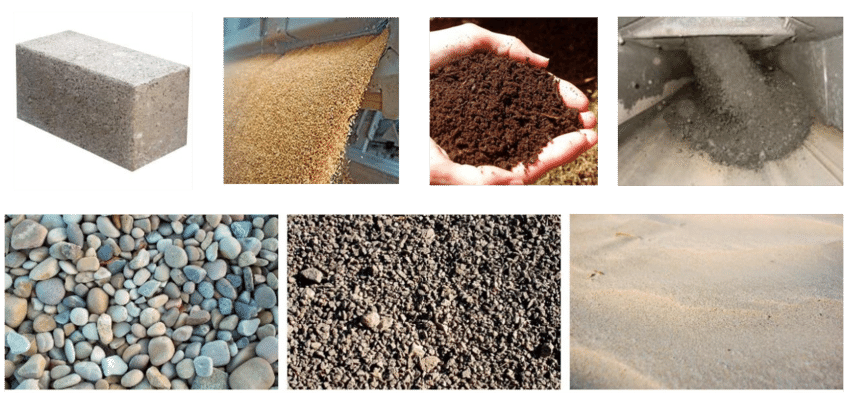
\includegraphics[scale=0.5]{granularExample.png}
    \caption{Examples of Granular Materials.\cite{granularExample}}
    \label{fig:granularExample}
\end{figure}

Granular material is a family of material characterized by its large bulk of densely packed particles, ranging from nanometers to centimeters \cite{introGranular2}, and is able to resist deformation and form heaps, i.e., behave like a solid and withstand strong shear force \cite{introGranular3}. Simple examples of granular materials include sand, gravel, clays, seeds, nuts, and all ranges of powders such as coffee powder, cement powder, which is shown in figure \ref{fig:granularExample}. Furthermore, many processes and equipments in chemical plants use granular materials, such as catalysis, adsorption, and heat exchangers. Granular materials are projected to make about half of the products and three-quarters of the raw materials used in the chemical industry \cite{introGranular}. Thus, understanding how granular materials behave is of great significance. 

The simulation of granular material's bulk mechanical behavior is done using Discrete Particle Model (DPM, or Discrete Element Method - DEM), which generates the movement of individual particles to capture the macro-scale behavior. The DPM is a family of numerical methods for computing the motion of a large number of particles \cite{Weng:2015}, first proposed by Cundall and Strack in the 1970s \cite{cundallstrack}.
Since the properties of granular materials differ wildly, these simulations require an extensive calibration process designed individually for each type of granular material. Some parameters of the granular material model can be measured directly, such as size distribution or density. However, other parameters are effective parameters (i.e., they result from a simplified particle model) and thus cannot be directly measured. These parameters are then calibrated by choosing a few standard calibration setups (rotating drum, heap test, ring shear cell) and simulating these setups in a DPM simulation, and the missing parameters are determined such that the response of the experimental and simulation setups match.

Recently, coupled with the raise of Machine Learning in other fileds, it has also been applied to solve the calibration problem. This has been done using a Neural Network \cite{nn-calibration, NN-GA, NN-coarse, YE2019292}, Genetic Algorithm \cite{ga-calibration}, and a recursive Bayesian sequential Monte-Carlo filtering algorithm named GrainLearning \cite{grainLearning}. In this Assignment, two Machine Learning algorithms will be discussed: Neural Network and GrainLearning. 

%todo is this true? 

These two algorithms set to treat the calibration problem in two different ways, and likewise, solve it in two different ways: While GrainLearning looks to identify the microparameters from the experimental and DEM simulations's bulk parameters (inverse problem), the Neural Network will help generating a database that can map different microparameters combinations to their corresponding bulk parameters, generated by DEM simulations. In other word, NN will learn the built-in relationship between the micro- and macroparameters of the Discrete Particle Model, thus allow a much faster prediction compare to a full DEM simulation. 
One advantage of GrainLearning compares to other Machine Learning algorithms such as Neural Network is that it is an unsupervised learning algorithm, i.e., it can starts calibrating with a minimal amount of input information. A normal calibration routine, currently implemented in MercuryDPM would only need the measurements data, parameter range, and the importance weight of each measurement (depends on the modeller's knowledge). Meanwhile, the current approach mentioned in \cite{nn-calibration, NN-GA, NN-coarse} would requires modeller to define a different NN model for each material, train it using a set of DEM simulations, and then validate the correct combinations of input-output by experiment. And although this process can be automated, to date the author has not been aware of any study implemented a fully-automated calibration routine using Neural Network. 


 \textbf{todo here: A paragraph describes each section}




% \section{Timeline and procedure}

% \subfile{TimelineSections/Timeline.tex}

% \section{Rebuttal}

% \subfile{RebuttalSections/Rebuttal.tex}


\section{Characterisation of granular materials}


There is no established standard of characterization measurements for granular materials. Typical measurements include heap test, rotating drum test, linear/ring shear cell test, and the silo flow test..., in which the output is the bulk parameter, which defines how the granular material behaves in large quantity~-~such as the angle of repose (AoR), shear stress, flow rate. 

This research is focused on one of the essential bulk parameters to describe the characteristics of the granular materials~-~the static angle of repose. Static AoR, described in Fig.~\ref{fig:StaticAoR}, is defined as the angle that granular solids form when piled with a flat surface and is essential to characterize the coarseness and smoothness of materials. This, in turn, can help design a process involved with the material~-~lower static AoR implies more flowable and thus easier to transport with less energy~\cite{TEFERRA201945}.

\begin{figure}[H]
    \centering
    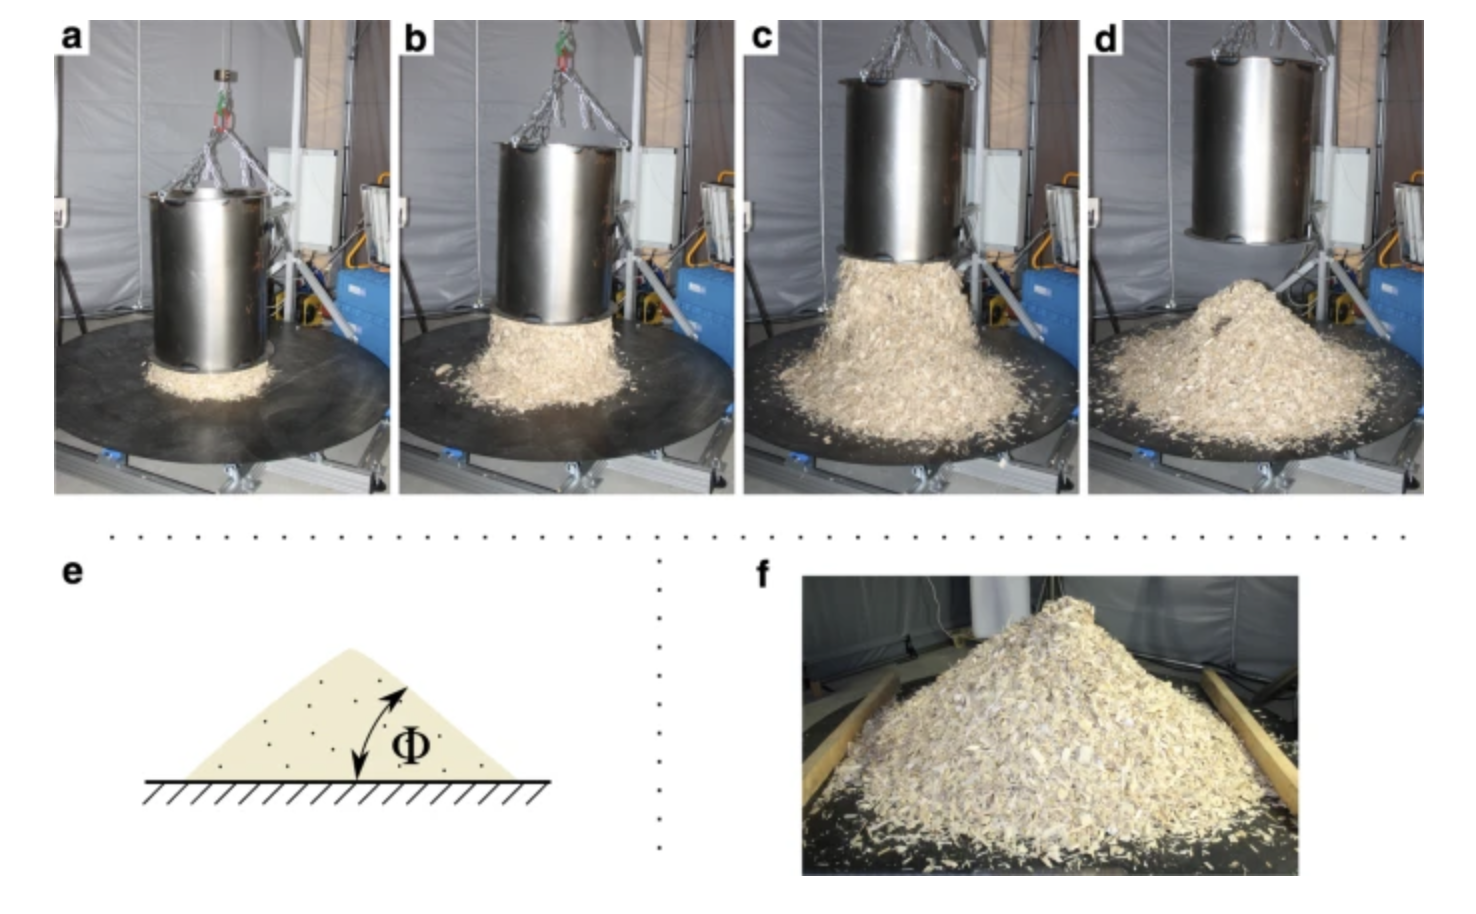
\includegraphics[scale=0.5]{StaticAoR.png}
    \caption{Static Angle of Repose measurement steps~\cite{Rackl:2018te}.}\label{fig:StaticAoR}
\end{figure}





\section{Simulation Method}\label{section:ExpMethod}


The DEM package used in this Assignment is MercuryDPM. MercuryDPM is an open-source DEM software package, developed by Thomas et al.\cite{MercuryDPM}. 






\subsection{Material and simulation properties}\label{section:matprop}

% Experimental data on quartz sand is provided by Derakhshani et al.~\cite{DERAKHSHANI2015127}. There is no specific intrest regarding the choice of material; quartz sand is chosen due to the availability of data and the similarity of measurements. The density of quartz sand is $\rho = 2653~kg/m^3$, and the particle size distribution (PSD) given in Table~\ref{table:PSDQuartzSand},. Static AoR of quartz sand measured by Derakhshani et al.~is $33^{\circ}$. Meanwhile, experimental data on limestone is provided by Shi et al.~\cite{SHI2020183}, specifically the Eskal 150 limestone, since this material has a similar experimental static AoR and density, while the PSD is in a much lower range. The density of Eskal 150 is $2761~kg/m^3$, and the static AoR is also $33^{\circ}$.


\begin{table}[H]
    % \centering\
    \begin{tabular}{l|l}
        Diameter (µm) & Cumulative Distribution (\%) \\ \hline
        300                    & 6.21                         \\
        425                    & 24.50                          \\
        500                    & 50.55                        \\
        600                    & 100                         
    \end{tabular}
    \begin{tabular}{l|l}
        Diameter (µm) & Cumulative Distribution (\%) \\ \hline
        97                    & 10                         \\
        138                    & 50                          \\
        194                    & 90                        
    \end{tabular}
    \caption{Particle Size Distribution of Eskal 150}\label{table:PSDlimestone} 
    \caption{Particle Size Distribution of quartz sand}\label{table:PSDQuartzSand}

\end{table}

\textit{The above tables will be fixed.}

% \begin{table}[H]
%     \centering
%     \begin{tabular}{l|l}
%         Particle Diameter (µm) & Cumulative Distribution (\%) \\ \hline
%         97                    & 10                         \\
%         138                    & 50                          \\
%         194                    & 90                        
%     \end{tabular}
%     \caption{Particle Size Distribution of Eskal 150}\label{table:PSDlimestone}
% \end{table}


The experimental data described above will be used as constant input values for each DEM simulation. In addition, four variables will be tested to determine their respective static AoR:\@
\begin{itemize}
    \item Restitution coefficient: Ratio between the velocity of the particle before and after collision.
    \item Sliding friction: Force that acts on the opposite direction of the movement between two particles when they collide. 
    \item Rolling friction: Force resists the rolling motion of the particle. 
    \item Bond number: Ratio between gravitational force that act on the particle and the surface tension force, i.e., the easiness of movement due to gravity. 
\end{itemize}







\section{Calibration of Discrete Particle Model}\label{section:Calibration}
    
\subsection{GrainLearning}\label{section:GLtheory}
GrainLearning is a calibration toolbox developed by Cheng et al., utilizes the recursive Bayesian algorithm to estimate the uncertainty parameters in DPM. Initially, a wide range of parameter space is quasi-randomly sampled from the initial guess range to create a prior distribution of each parameter. Then, conditioned on the experimental values, the posterior distribution of the parameters is updated recursively by Sequential Monte-Carlo Filtering (SMC Filter) and fitted to a Gaussian Mixture Model. This process is done iteratively, until a desired value that minimises the loss function is reach, typically 3 iterations. Algorithm \ref{algorithm:GrainLearning} and the following sections will describe in brief the calibration workflow implemented in GrainLearning. 

\begin{algorithm}
    \caption{GrainLearning}\label{algorithm:GrainLearning}
    \begin{algorithmic}
        \State$\textbf{Input:}$
        \State$\hspace*{5mm}\text{\textbf{y: }} \text{Experimental values} $
        \State$\hspace*{5mm} \textbf{x = F$(\Theta)$} \text{: DEM solver}$
        \State$\hspace*{5mm}(\Theta_{min}, \Theta_{max}) \text{: Initial guess range} $
        \State$\textbf{Main:}$

            \LineComment{\textit{Set uniform prior distribution:}} $p(\Theta) = \mathcal{U}(\Theta_{min}, \Theta_{max})$
            \For{k in range $(0, K)$}
                \LineComment{\textit{Sampling parameters: }}
                \If {$k = 0$} $\text{sample $N_{p}$ parameters values from initial  distribution: } \Theta_{k}^{(i)} \sim p_0(\Theta) $
                \ElsIf {$k > 0$} $\text{sample $N_{p}$ parameters values from prior distribution: } \Theta_{k}^{(i)} \sim p_{k-1}(\Theta \mid y_{1:T})$
                \EndIf
                % \State$\text{Assume the normalized covariance parameter } \sigma $
                \LineComment \textit{Evaluate DPM: }  $x_{k}^{(i)} = F(\Theta_{k}^{(i)}) $ 
                \LineComment{Optimizing $\sigma$: }
                \While{$\text{True}$} 
                    \LineComment{\textit{Compute likelihood (Eq. \ref{eq:likelihood}): }} $p(y_t \mid \Theta_{k}^{(i)} ) \propto \mathcal{N}(y_{kt} \mid x_{kt}^{(i)}, \Sigma)$ 
                    \LineComment{\textit{Compute posterior distribution of of $\Theta_{k}^{(i)}$ conditioned to $y$ (Eq. \ref{eq:posterior}).}}
                    \LineComment{\textit{Compute Effective Sample Size (ESS) with Eq. \ref{eq:ESS}}.} 
                    \LineComment{\textit{Stop if target ESS value is reached: }} 
                    \If {$k = 0 \text{ and } ESS > 20\%$} $\text{break}$
                    \ElsIf{$k > 0 \text{ and } ESS \sim ESS_{max}$} $\text{break}$
                    \EndIf
                \EndWhile
                \LineComment{\textit{Fit sampled posterior distribution to Gaussian Mixture Model: }}  
                $p(\Theta \mid y) = \sum_{\alpha}^{k} \lambda_{\alpha} \mathcal{N}(\mu_{\alpha}, \sigma_{\alpha}) $
                \LineComment{\textit{Set new prior distribution: }} $p(\Theta) \gets p(\Theta \mid y)$
            \EndFor
        \State \textbf{Output: } $\Theta_{opt}$ in $\Theta_{K}$ that minimizes $|F(\Theta_{opt} - y)|$
    \end{algorithmic}
\end{algorithm}

\subsubsection{Posterior distribution calculation}


Initially, the measurement is assumed to have an error represented by a covariance matrix $\Sigma_{\alpha} = \sigma\omega_{\alpha}y_{\alpha}$, with $\sigma$ the covariance parameter, and important weight of the measurement $\omega$. With $\Sigma$, the likelihood of a given state $\Theta_{k}^{(i)}$, i.e., the probabilistic prediction to the experimental data $y$ can be estimated by the multivariate normal distribution, with $y_t$ measurement data at time step t, and $d$ the dimension of the state vector $\Theta_{k}^{(i)}$:


\begin{equation} \label{eq:likelihood}
p(y_t \mid \Theta_{k}^{(i)}) \propto \frac{1}{(2\pi)^{d/2}|\Sigma|}exp\left(-\frac{1}{2}(y_{kt} - x^{(i)}_{kt})^{\mathsf{T}}\Sigma^{-1}(y_{kt} - x^{(i)}_{kt} )\right)
\end{equation}

With the calibration system being modelled as a hidden Markov model, the posterior distribution of $\Theta_{k}^{(i)}$ can be calculated using recursive Bayes' rule: 

\begin{equation} \label{eq:posterior}
    p(\Theta_{k}^{(i)} \mid y) \propto \prod_{t=1}^{N_{t}} p(y_t \mid \Theta_{k}^{(i)} )p( \Theta_{k}^{(i)} ) 
\end{equation}

\subsubsection{Effective multi-level sampling}

The Effective Sample Size (ESS) is calculated by summing the posterior distribution squared of all the sampled parameters value $N_{p}$:

\begin{equation} \label{eq:ESS}
ESS = \frac{1}{N_{p} \sum_{i=1}^{N_{p}} p(\Theta_{k}^{(i)} \mid y)^2}
\end{equation}

The main idea is to draw the sample from the previously acquired knowledge about the relationship between $\Theta$ and $y$. In the first iteration ($k = 0$), The uniform prior distribution is chosen as the proposal density, and the parameter spaces are drawn from there. Subsequently, for $k > 0$, the proposal density will be the posterior distribution from the previous iteration $p(\Theta \mid y)$. After each iterations, the sampling space will get narrower~-~therefore, to ensure a proper proposal density for the sampling of parameters, the optimization process will be continued until appropriate $\sigma$ which maximizes ESS is reached. 

\subsubsection{Identification of microparameters with GrainLearning}
In the first iteration of calibration, GrainLearning will initialize a set of parameter combinations using Halton sequence, from the initial guess range provided. This set of parameters will be passed to MercuryDPM to analyze with a Heap test, after which a static AoR is produced. From this data, GrainLearning will compute the next set of parameters on the basis of the previous MercuryDPM output, according to algorithm~\ref{algorithm:GrainLearning}. For each attempt, GL will be running for 4 iterations~-~except when the simulations of that iteration takes more than two days, and that attempt will be classified as failed. 




    


\subsection{Neural Network}
\documentclass[../BachelorAssignment.tex]{subfiles}
    

\begin{document}
\graphicspath{{\subfix{../Images/}}}

Artificial Neural Network (ANN) is a set of algorithms that seeks to identify correlations in data utilizing a technique that inspired by the way human brain operates - mimicking how each neurons in the brain signaling each other. The most basic ANN models is the Feedforward Multilayer Perceptron Neural Network (MLPNN), in which the purpose is to define the mapping between the input and output \(y = f(x;\theta)\), and approximate the parameter \(\theta\) which results in the best possible function. In MLPNN, the data will flows in one direction from the input to output, hence the name feedforward. Like other supervised learning algorithms, a MLPNN need to be trained before it can accurately describe the relations between the input and output. This is typically done by feeding the network with pre-labeled data, compare the model's output with the desired output, and update the weights parameter \(\theta\) - a process called backpropagation. In the context of this Assignment, Neural Network (NN) will be used when refering to Feedforward Multilayer Perceptron Neural Network. 



In order to choose a correct NN model that can describes the relationship of micro- and macroparameters as indicated in the contact law, a "bottom-up" method is employed. Initially, a simple one-input one-output NN will be built, to assess how many layers (and neurons) it would take to learn a quadratic relationship \(y = x^2\), and inverse relationship \(y = 1/x\).

In the next step, a slightly more complex problem is analysed: a 4-D input and 4-D output model, with contact laws described in table xxx. Finally, a fully-functional model will be coupled with DEM simulations from MercuryDPM.   

Certain reccomendations will also be taken into account, (7 and 15? )


\end{document}

\subsection{Random Forest algorithm}

This section will discuss different concepts of a Random Forest (RF) algorithm, starting with the basis of the RF:\@ decision tree. Decision tree is an algorithm that generates a tree graph of decisions based on the input provided and their possible outcomes, and as a consequence, it partitions the input space into multiple regions, with each region accounting for a different outcome~\cite{murphyML}. An example of a simple decision tree based on two inputs is shown in figure~\ref{fig:decisionTree}. 

\begin{figure}[H]
    \centering
    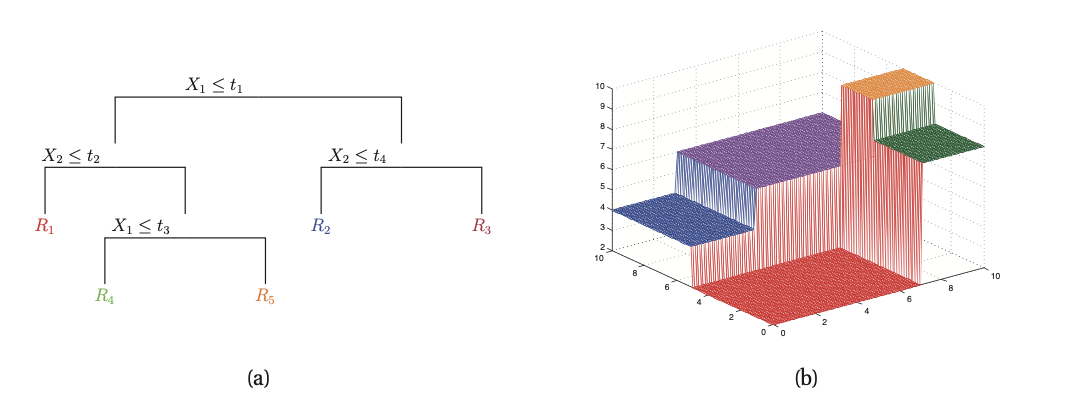
\includegraphics[scale=0.8]{regressionTree.png}
    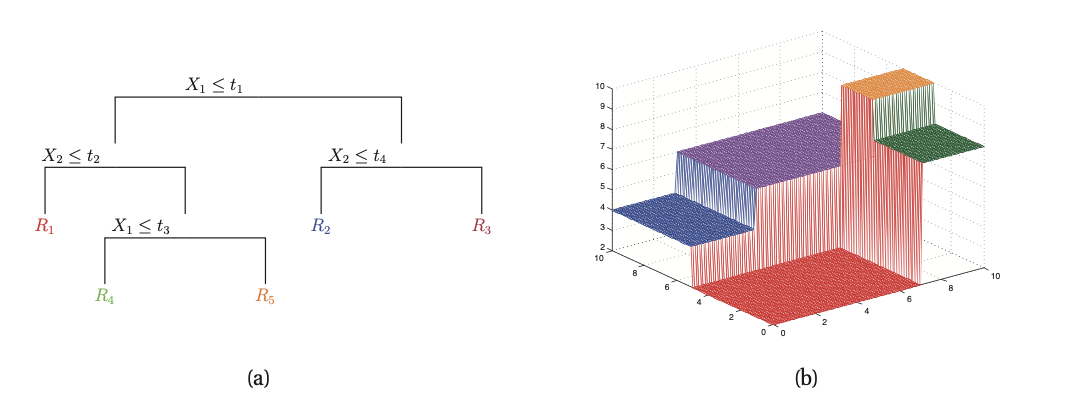
\includegraphics[scale=0.8]{decisionTree.png}
    \caption{Example of a decision tree regressor on a two-input problem.~\cite{murphyML}}\label{fig:decisionTree}
\end{figure}

The most significant advantage of the decision tree, and subsequently, random forest algorithm, is that it is relatively simple, explainable, easy to train and interpolate with little computational resources. However, one crucial drawback of a decision tree is its instability: minor data changes might affect the tree structure, making the decision tree a high variance estimators~\cite{murphyML}. Attempts have been made to reduce the uncertainty of the decision tree, one of which is the so-called Random Forest algorithm, which Breiman proposed in 2001~\cite{BreimanRF}. RF made up for the high variance of a single decision tree by averaging the results over a ``forest'' of decision trees, with each tree represents an independent sampled vectors. The concept of decision tree and RF, therefore, fit within the scope of the calibration problem.


\subsection{Training and evaluation method for supervised models}  

To train the NN and RF model, 500 DEM simulations with randomized combinations of input parameters have been performed, in order to create a database which maps DEM microparameters to static AoR. Other 125 simulations did not finish on the time constraint set, and as a results marked as an inaccurate combination. 




\input{MaterialandSimulation/CalibrationMethod.tex}

% section result and analysis 

\section{GrainLearning evaluation}\label{section:GLPerformance} 
 
This section discusses the calibration results for quartz sand and limestone's static AoR with GrainLearning. For each material, calibration was performed in three different attempts, with the difference between each attempt being the search range specified (see table~\ref{table:GLCalibration}), i.e., GL will try to sample different combinations in the first iteration within that range. In the first attempt, the search range was in the default setting, and the second and third attempts will be adjusted according to the first result.

\begin{table}[H]
    \centering
    \begin{tabular}{l|lll|lll}
    Material                & \multicolumn{3}{l|}{Quartz Sand}       & \multicolumn{3}{l}{Limestone}          \\ \hline
    Attempt                 & 1          & 2           & 3           & 1          & 2           & 3           \\ \hline
    Restitution Coefficient & {[}0.5  1{]} & {[}0  1{]}  & {[}0 1{]}   & {[}0.5  1{]} & {[}0.5  1{]}  & {[}0 1{]}   \\
    Rolling Friction        & {[}0 1{]}  & {[}0 0.5{]} & {[}0.5 1{]} & {[}0 1{]}  & {[}0 0.5{]} & {[}0.5 1{]} \\
    Sliding Friction        & {[}0 1{]}  & {[}0 0.5{]} & {[}0.5 1{]} & {[}0 1{]}  & {[}0 0.5{]} & {[}0.5 1{]} \\
    Bond number             & {[}0 1{]}  & {[}0 0.5{]} & {[}0.5 1{]} & {[}0 1{]}  & {[}0 0.5{]} & {[}0.5 1{]} \\
    \end{tabular}
    \caption{Calibration attempts using GL}\label{table:GLCalibration}
\end{table}


\subsection{Limestone}
The calibration results by GL for limestone are described in table~\ref{table:resEskalGL}, and the details on how the sampling algorithm performs, i.e., conditioned on the previous simulation, is the sampled parameters for the next iteration make the simulation result converge to the experimental result, are described in figure~\ref{fig:EskalGL}. In the third calibration attempt, the second iteration did not finish in time due to the system's high level of kinetic energy; therefore, only iteration 1 is shown. 

In the first attempt, only four iterations were performed initially. However, one remarkable observation is that GL clusters over the combinations produce a static AoR around $40^{\circ}$. This is reflected in the second iteration's result, where the best combination results in a static AoR of $39.4803^{\circ}$. Moreover, although the third iteration's result is $33.0979^{\circ}$, this seems like an outlier of the cluster. Consequently, an additional iteration was performed~-~and the results here verify the observation. The closest value to experimental static AoR is $31.5243^{\circ}$, and it is also an outlier. 

After the first calibration attempt, it is clear that the combinations that would result in the desired static AoR lie around $0.8-1.0$ for restitution coefficient and in the lower-0.25 range for the rest of the contact parameters. Therefore, two more attempts were performed, with different initial ranges: attempt 2 with sliding friction, rolling friction, and bond number ranging from 0 to 0.5. With attempt 3, the sliding friction, rolling friction, and bond number range from 0.5 to 1, while the restitution coefficient's range is widened to 0 to 1. 

As expected, the second attempt's performance was the most robust, reaching a near-perfect solution at the end of iteration 4. The clustering of the optimal result can also be seen clearly in figure~\ref{fig:EskalGL}. Meanwhile, the results from the third attempt verify the conclusion from the first attempt about the range of the optimal parameters~-~with higher rolling friction, sliding friction, and bond number, the static AoR reaches a maximum value of around $65^{\circ}$.

\begin{figure}[H]
    \centering
    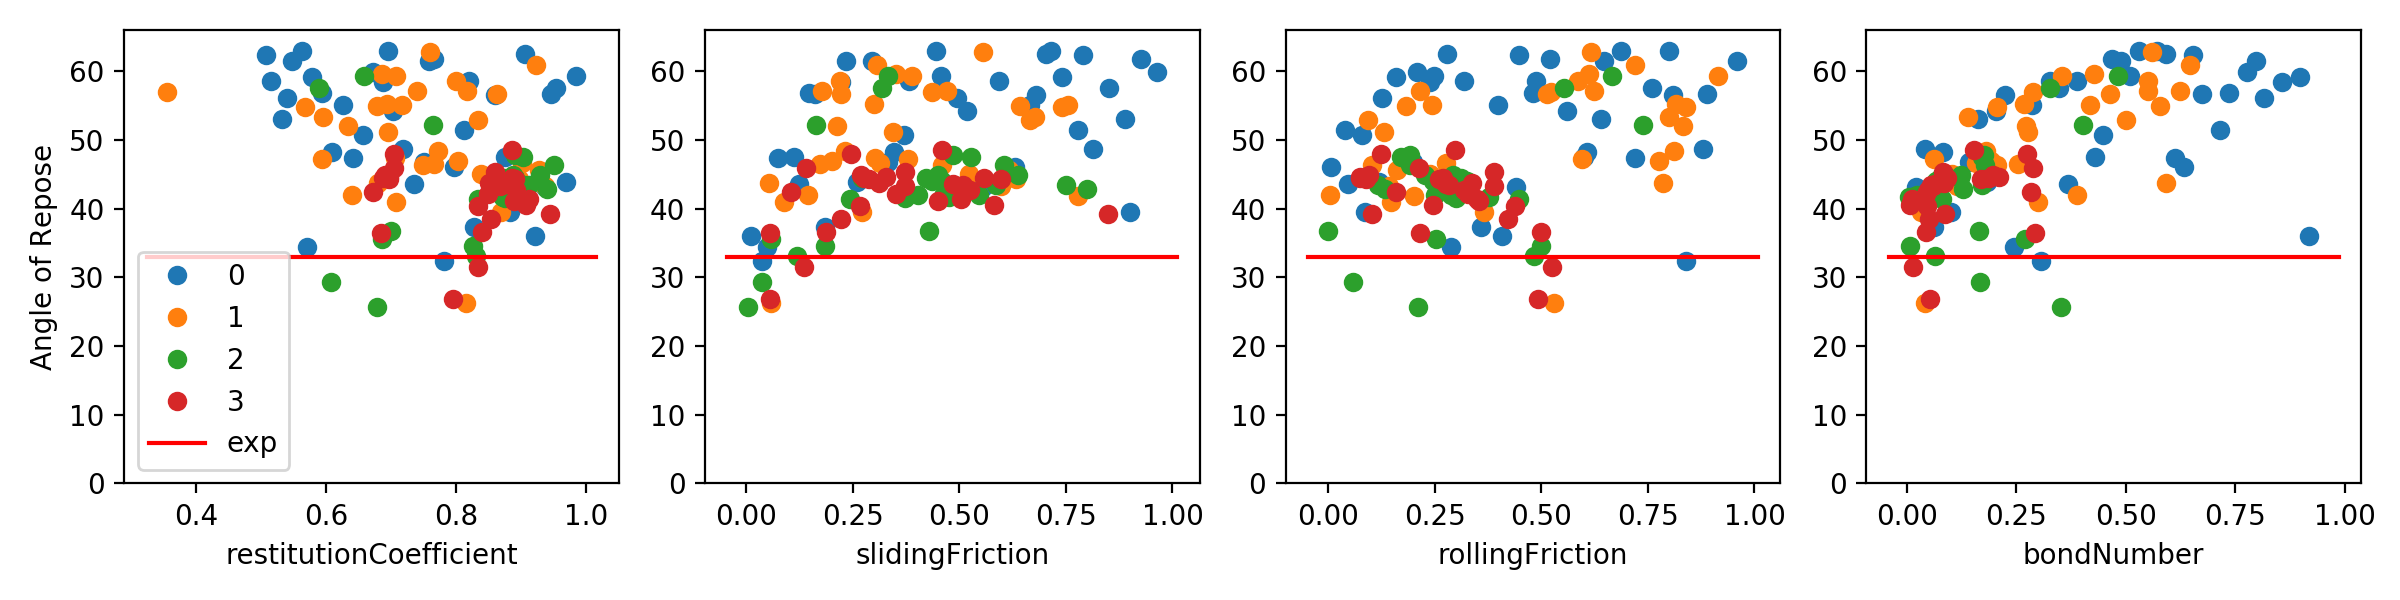
\includegraphics[scale=0.51]{ParametersObserver_Eskal150.png}
    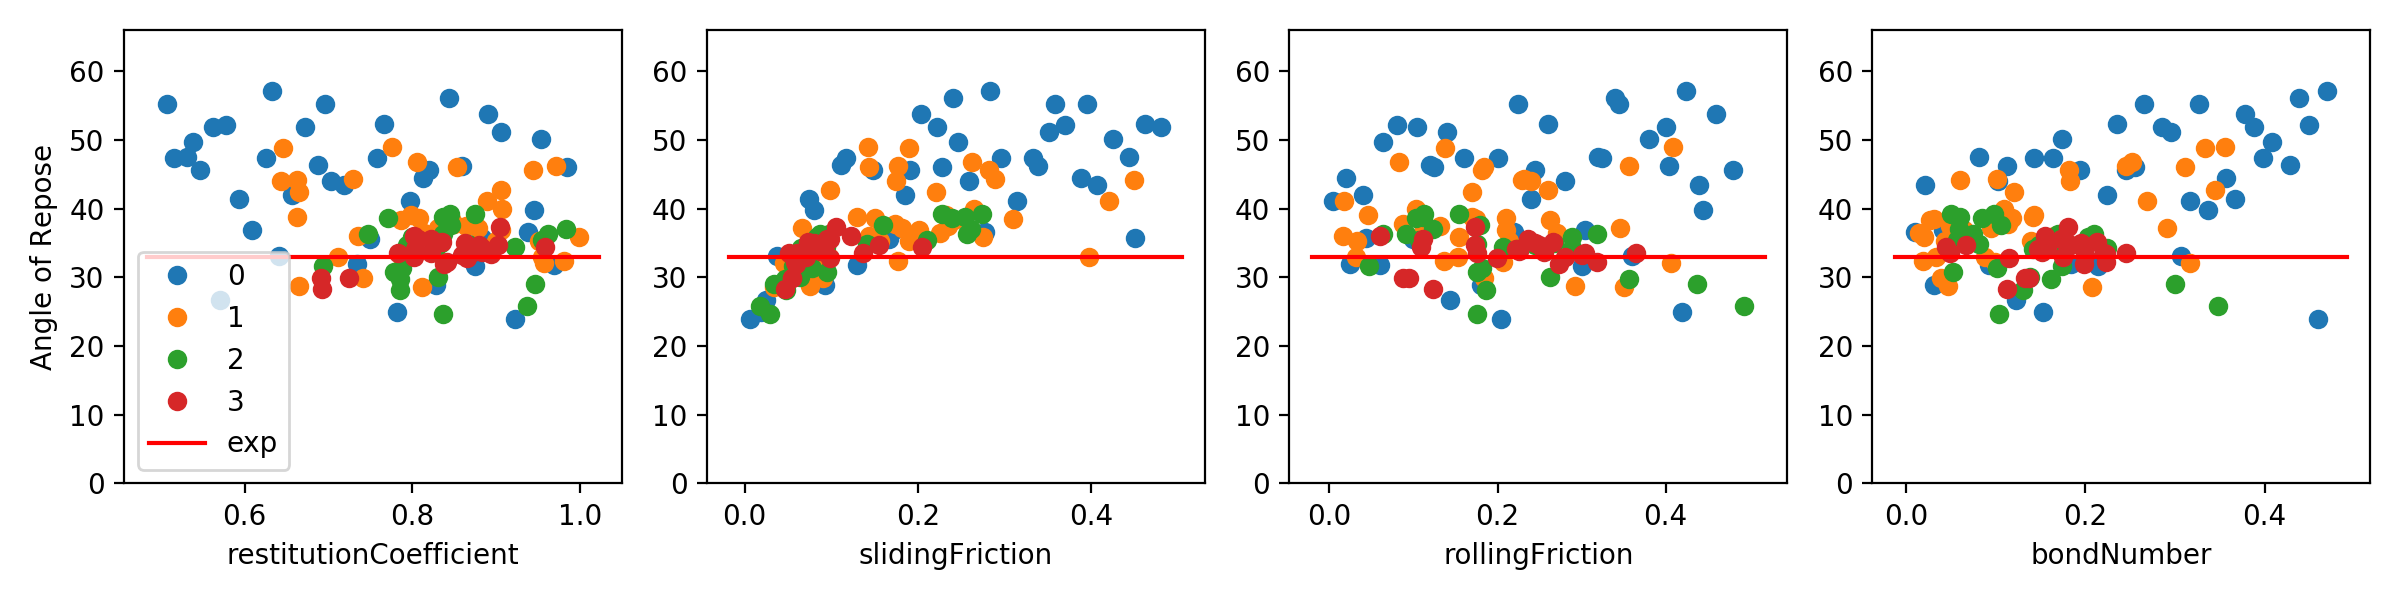
\includegraphics[scale=0.51]{ParametersObserver_Eskal150_1.png}
    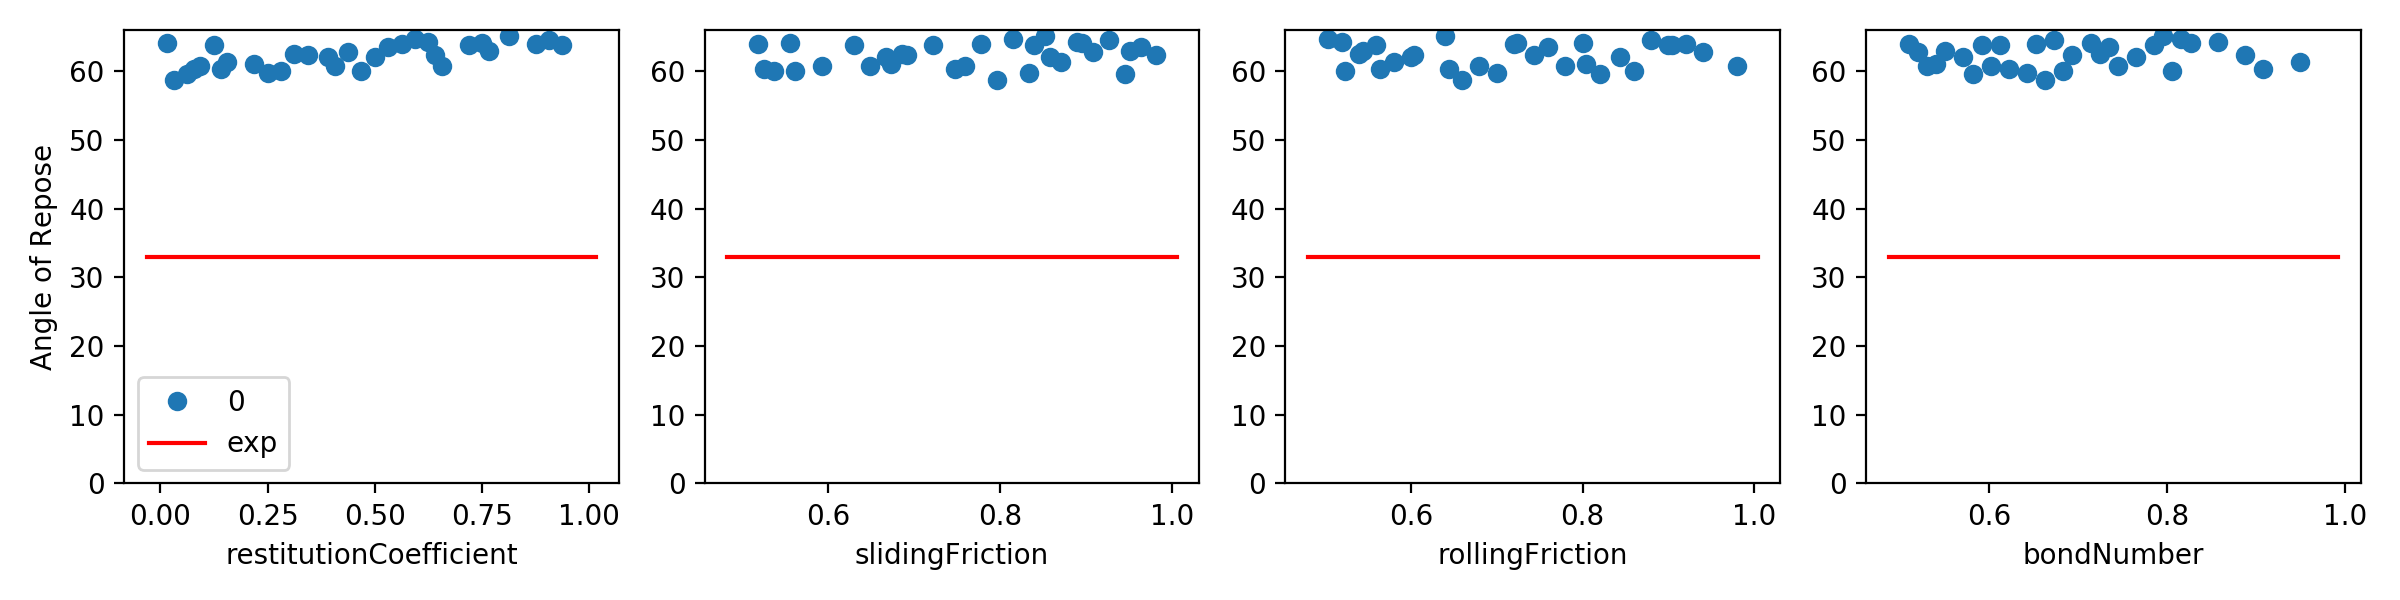
\includegraphics[scale=0.51]{ParametersObserver_Eskal150_2.png}
    \caption{\textit{From top to bottom,} attempt 1, 2, and 3 at calibrating Eskal with GL.\@ Scatter dots with different colors denote each iteration, and red line denotes experimental value.}\label{fig:EskalGL}
\end{figure}
    
\begin{table}[H]
    \centering
    \resizebox{\textwidth}{!}{%
    \begin{tabular}{c|ccccc}
    Attempt/Iter & Restitution Coefficient & Sliding Friction & Rolling Friction & Bond number & Result AoR \\ \hline
    1.1 & 0.7812 & 0.037 & 0.84 & 0.3061 & 32.3163 \\
    1.2 & 0.869 & 0.2725 & 0.3652 & 0.0325 & 39.4803 \\
    1.3 & 0.831 & 0.1194 & 0.484 & 0.064 & 33.0406 \\
    1.4 & 0.8332 & 0.135 & 0.5262 & 0.0137 & 31.5243 \\
    1.5 & 0.8348 & 0.1517 & 0.497 & 0.0297 & 33.6745 \\
    2.1 & 0.6406 & 0.037 & 0.36 & 0.3061 & 33.0979 \\
    2.2 & 0.9546 & 0.3983 & 0.032 & 0.0334 & 32.9993 \\
    2.3 & 0.8263 & 0.0917 & 0.2226 & 0.1411 & 34.1421 \\
    2.4 & 0.8025 & 0.0710 & 0.2802 & 0.1748 & 32.9812 \\
    3.1 & 0.0312 & 0.7963 & 0.66 & 0.6632 & 58.6606
    \end{tabular}%
    }
    \caption{Calibration results of limestone with GL.}\label{table:resEskalGL}
\end{table}

\subsection{Quartz sand}

The calibration result for quartz sand is given in table~\ref{table:resSandGL}, and the parameters sampling graph is given in figure~\ref{fig:QuartzGL}. In the control attempt, only the first iteration is shown, partly due to 6/40 simulations of the second iteration does not finish in time, but also due to the results of the second iteration does not cluster at the experimental value, with most averaging around $45^{\circ}$ to $50^{\circ}$. Due to the similarity between quartz sand and limestone in terms of experimental static AoR, the second attempt of quartz sand will be initialized with the same range as the second attempt of limestone. And as a result, attempt 2 has the best performance out of the three. One noticeable thing here is that the rolling friction has two different clusters identified by GL instead of one, compared to sliding friction, restitution coefficient, or bond number. This denotes the multi-solution phenomena of a calibration problem since there could be more than one combination that can produce a sufficient static AoR~-~which is shown in iterations 3 and 4 of attempt 2: the rolling friction for iteration 3 is 0.07, while for iteration 4 is 0.41. Different experiments, i.e., Shear Cell test or Drum test (Dynamic AoR), would be needed in addition to the heap test to find an ideal combination of microparameters. However, this is out of the scope of the current research. 

In the third attempt, although the range was specified as shown in table~\ref{table:GLCalibration}, the Gaussian Mixture Model algorithm of GL sampled some of the values in iteration 3 and 4 outside the initial range. This was a known bug in the current GL version implemented in MercuryDPM. Therefore, it was able to generate a correct combination with very low sliding friction, which results in a static AoR of $34.2227^{\circ}$, remarkably close to the experimental value. 


\begin{figure}[H]
    \centering
    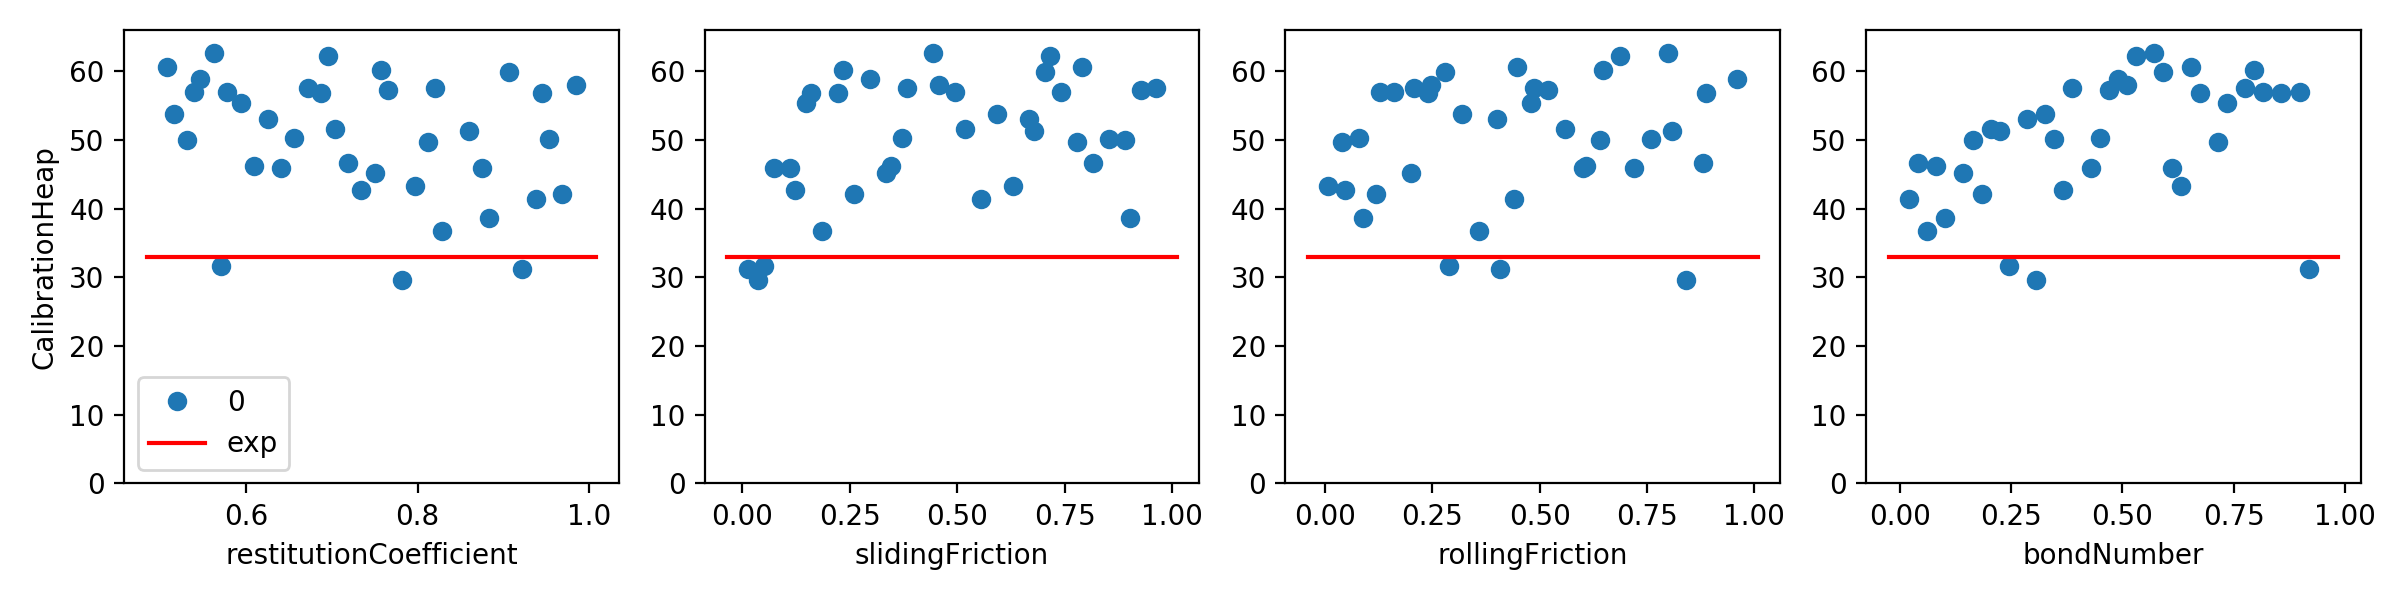
\includegraphics[scale=0.51]{ParametersObserver_SandHeap_copy.png}
    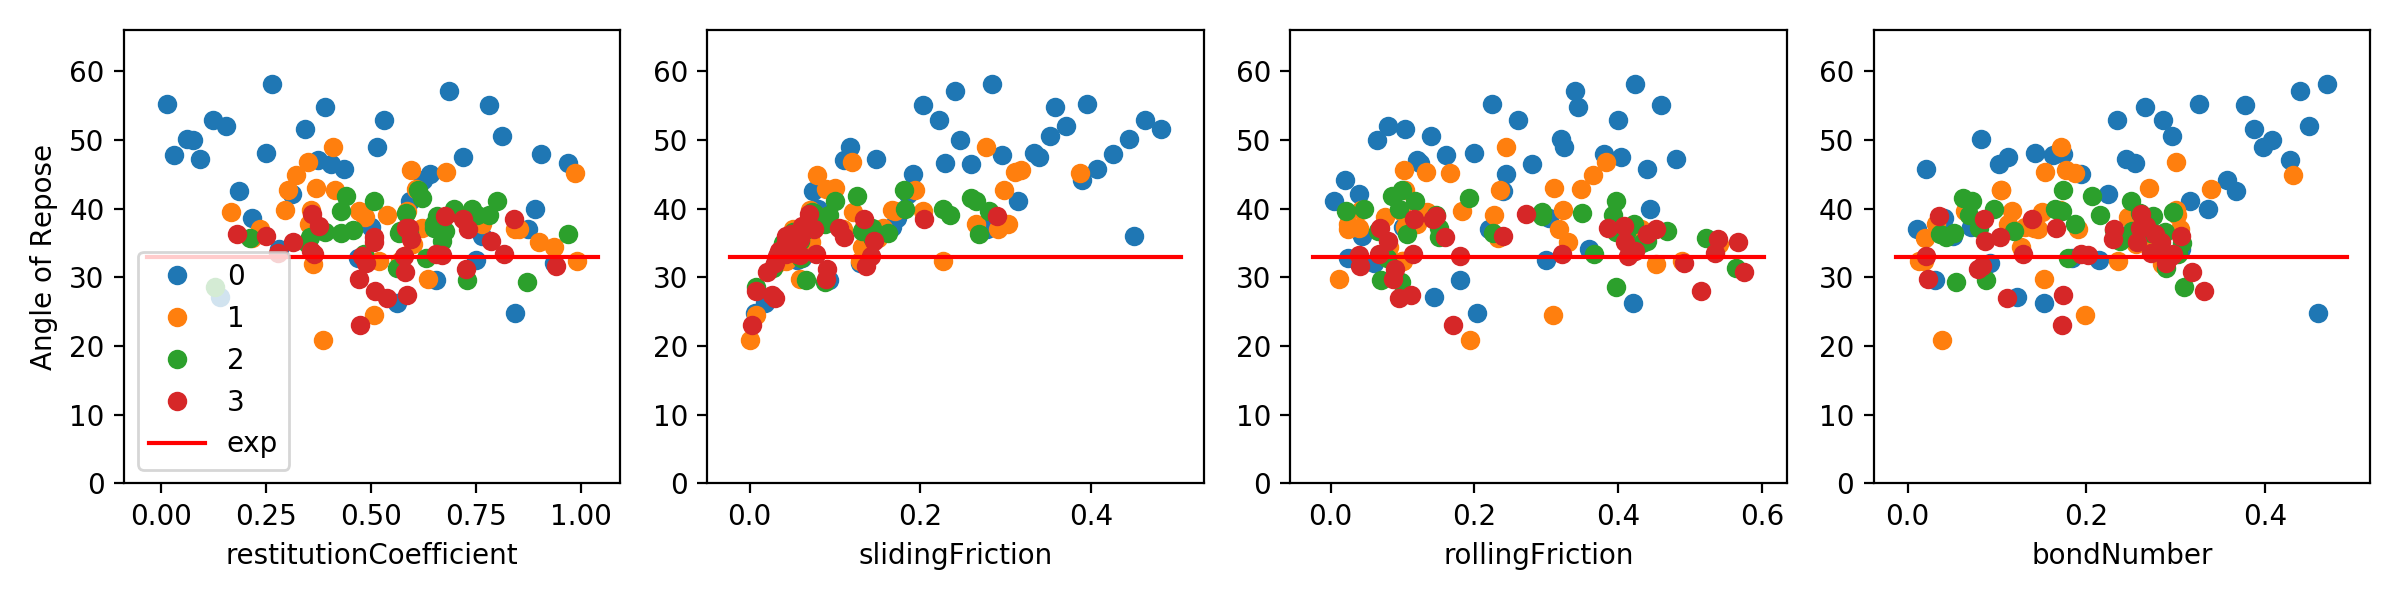
\includegraphics[scale=0.51]{ParametersObserver_Sand2.png}
    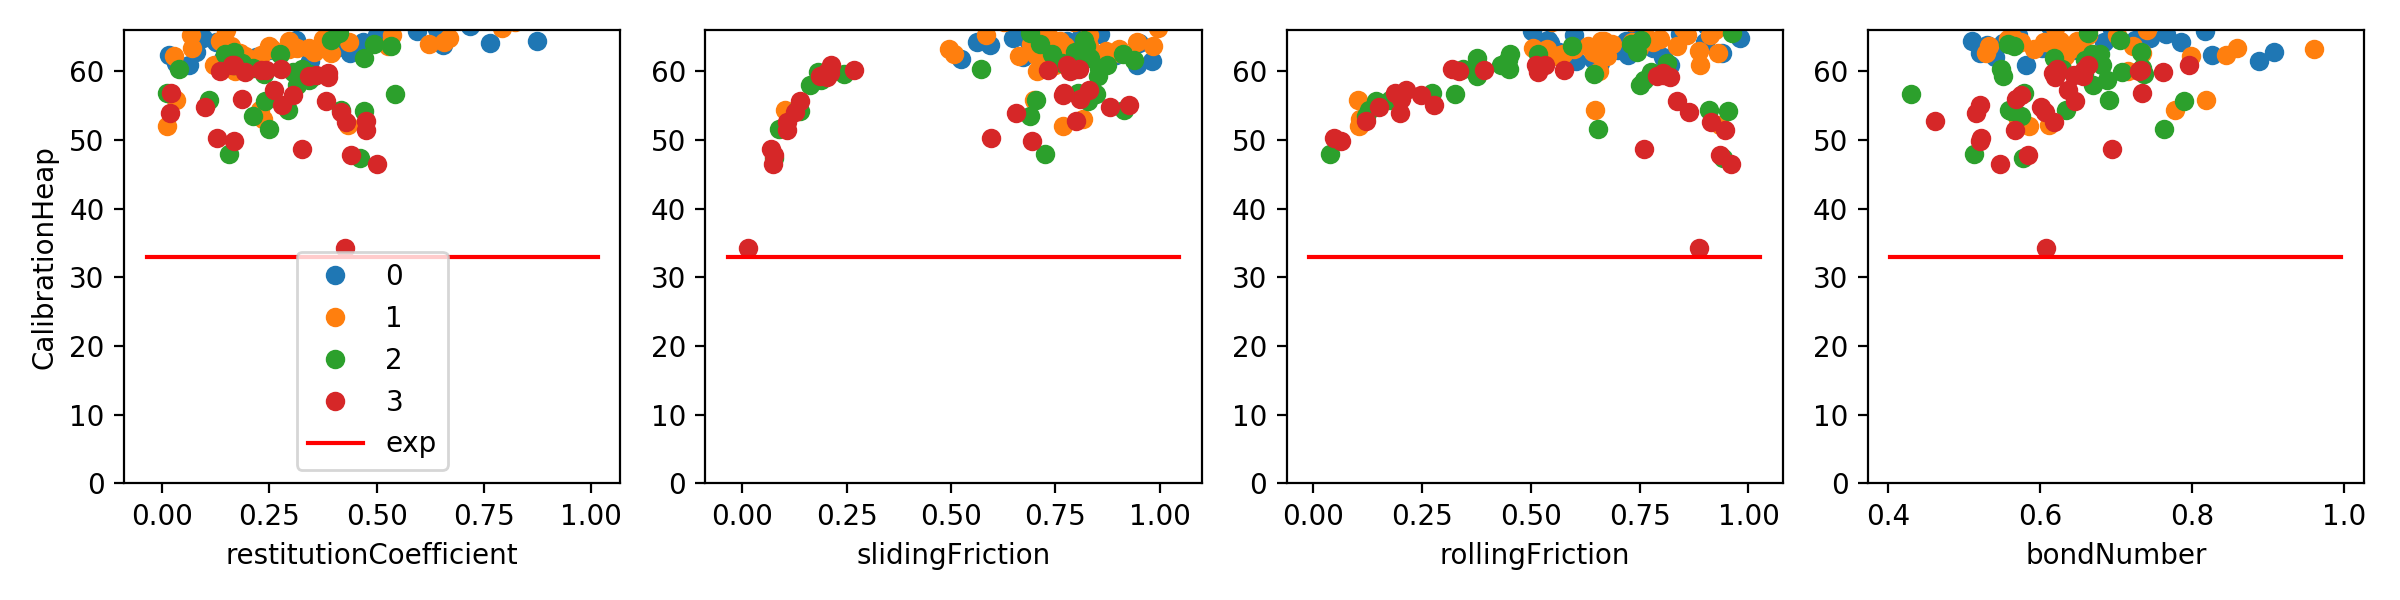
\includegraphics[scale=0.51]{ParametersObserver_Sand2_2.png}
    \caption{\textit{From top to bottom,} attempt 1, 2, and 3 at calibrating quartz sand with GL.\@ Scatter dots with different colors denote each iteration, and red line denotes experimental value.}\label{fig:QuartzGL}
\end{figure}

\begin{table}[H]
    \centering
    \resizebox{\textwidth}{!}{%
    \begin{tabular}{c|ccccc}
    Attempt/Iter. & Restitution Coefficient & Sliding Friction & Rolling Friction & Bond number & Result AoR \\ \hline
    1.1 & 0.5703 & 0.0493 & 0.288 & 0.2448 & 31.6303 \\
    2.1 & 0.4688 & 0.0617 & 0.024 & 0.1836 & 32.8394 \\
    2.2 & 0.992 & 0.2261 & 0.0987 & 0.0126 & 32.3687 \\
    2.3 & 0.6307 & 0.0606 & 0.0787 & 0.1795 & 32.8670 \\
    2.4 & 0.4800 & 0.0321 & 0.413 & 0.2946 & 33.0521 \\
    3.1 & 0.0625 & 0.9444 & 0.82 & 0.5816 & 60.9714 \\
    3.2 & 0.0109 & 0.7683 & 0.1052 & 0.5853 & 52.0551 \\
    3.3 & 0.4604 & 0.0752 & 0.9406 & 0.5777 & 47.3408 \\
    3.4 & 0.427 & 0.0146 & 0.8872 & 0.6075 & 34.2227
    \end{tabular}%
    }\caption{Calibration results of sand with GL.}\label{table:resSandGL}
\end{table}

\subsection{Discussion} 
 
Overall, GL has demonstrated the capability to identify the `cluster' in all calibration cases that the initial ranges were correctly defined~-~the combinations after each iteration are sampled closer and closer to the experimental value, as shown in attempt 2 of limestone and quartz sand. However, it has also shown inconsistent performance: In attempt 1 of limestone, the algorithm seeks to cluster in the range of $35^{\circ}$ to $45^{\circ}$. 


\section{Supervised model evaluation}\label{section:supervisedPerformance}

In this section, the performance of the two supervised models, i.e., Neural Network and Random Forest, is investigated for limestone and quartz sand, respectively. For the NN model, over 800,000 combinations, as described in table~\ref{table:randomCombinations}, have been processed~-~and over 2,000,000 for the RF model. Any combinations that produce a static AoR within the $0.1\%$ margin of error to the experimental data are marked as a correct combination. This combination will then be evaluated independently by a DEM simulation to verify the ability of supervised models to correctly describe a material's bulk behavior based on the given contact law. 

\begin{table}[H]
    \centering
    \resizebox{\textwidth}{!}{%
    \begin{tabular}{c|cccc}
     & Restitution Coefficient & Sliding Friction & Rolling Friction & Bond number \\ \hline
    Range & {[}0.5 1{]} & {[}1e-5 1{]} & {[}1e-5 1{]} & {[}1e-5 1{]} \\
    Number of values (NN) & 30 & 30 & 30 & 30 \\
    Number of values (RF) & 38 & 38 & 38 & 38
    \end{tabular}%
    }
    \caption{Random evenly-spaced microparameters combinations}\label{table:randomCombinations}
\end{table}
    
\subsection{Limestone}

For limestone, 12 over 800,000 combinations of DEM input parameters processed by the ANN was a `valid' combination: the output of the ANN was $33\pm 0.01^{\circ}$. Meanwhile, with 2,000,000 million combinations processed by RF, 22 of them were valid combinations~-~however, many of them are closely similar with a minor difference in one of the micro parameters, and only nine are distinct. The valid combinations are described in table~\ref{table:EskalNN} and~\ref{table:eskalRF}, with figure~\ref{fig:EskalNNRF} illustrates the combinations and their respective output. Overall, the NN model has correctly identified three combinations, while the Random Forest model has 2. 


\begin{figure}[H]
    \centering
    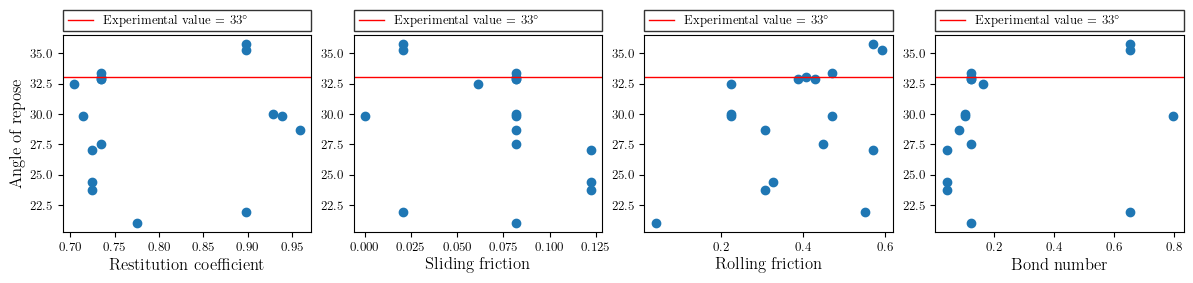
\includegraphics[scale=0.51]{rf_eskal.png}
    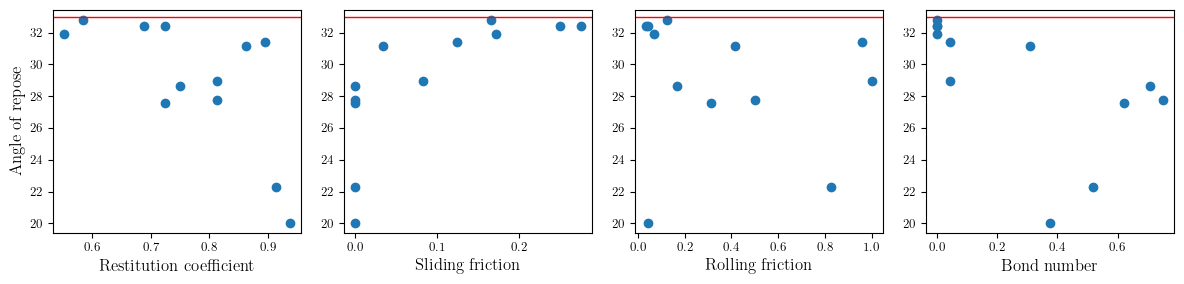
\includegraphics[scale=0.51]{nn_eskal.png}
    \caption{\textit{From top to bottom,} valid contact law parameters identified by Random Forest and Neural Network model for limestone, and their respective simulation results.}\label{fig:EskalNNRF}
\end{figure}

      
\begin{table}[H]
    \centering
    \resizebox{\textwidth}{!}{%
    \begin{tabular}{cccc|c}
    Restitution coefficient & Sliding friction & Rolling friction & Bond number & Angle of repose \\ \hline
    \textbf{0.6875} & \textbf{0.2500} & \textbf{0.0417} & \textbf{0} & \textbf{32.4263} \\
    0.7500 & 0 & 0.1667 & 0.7083 & 28.6156 \\
    \textbf{0.5833} & \textbf{0.1667} & \textbf{0.1250} & \textbf{0} & \textbf{32.7926} \\
    0.5517 & 0.1724 & 0.0690 & 0 & 31.9425 \\
    0.8125 & 0.0833 & 1.0000 & 0.0417 & 28.9393 \\
    \textbf{0.7241} & \textbf{0.2759} & \textbf{0.0345} & \textbf{0} & \textbf{32.3962} \\
    0.8958 & 0.1250 & 0.9583 & 0.0417 & 31.4044 \\
    0.8621 & 0.0345 & 0.4138 & 0.3104 & 31.1331 \\
    0.7241 & 0 & 0.3104 & 0.6207 & 27.5978 \\
    0.8125 & 0 & 0.5000 & 0.7500 & 27.7676 \\
    0.9138 & 0 & 0.8276 & 0.5172 & 22.2677 \\
    0.9375 & 0 & 0.0417 & 0.3750 & 20.0361
    \end{tabular}%
    }
    \caption{Valid contact law parameters identified by the NN model for limestone and their respective simulation results. }
    \label{table:EskalNN}
\end{table}
                
\begin{table}[H]
    \centering
    \resizebox{\textwidth}{!}{%
    \begin{tabular}{cccc|c}
    Restitution coefficient & Sliding friction & Rolling friction & Bond number & Angle of repose \\ \hline
    \textbf{0.7041} & \textbf{0.0612} & \textbf{0.2245} & \textbf{0.1633} & \textbf{32.4872} \\
    0.7245 & 0.1225 & 0.5714 & 0.0408 & 27.0585 \\
    \textbf{0.7347} & \textbf{0.0816} & \textbf{0.4082} & \textbf{0.1225} & \textbf{33.0331} \\
    0.7347 & 0.0816 & 0.4694 & 0.1225 & 33.3593 \\
    0.7755 & 0.0816 & 0.0408 & 0.1225 & 21.0172 \\
    0.8980 & 0.0204 & 0.5714 & 0.6531 & 35.7342 \\
    0.9286 & 0.0816 & 0.2245 & 0.1020 & 29.9625 \\
    0.9592 & 0.0816 & 0.3061 & 0.0816 & 28.6865 \\
    0.7143 & 0 & 0.4694 & 0.7959 & 29.8154
    \end{tabular}%
    }
    \caption{Valid contact law parameters identified by the RF model for limestone and their respective simulation results.}
    \label{table:eskalRF}
\end{table}


\subsection{Quartz Sand}

The quartz sand model was trained with fewer simulations compared to the limestone model, with 322 DEM simulations, partially due to more simulations with quartz sand cannot be complete. However, data from the completed simulations have shown that the uncompleted one would mainly result in a static AoR of $50^{\circ}$ or higher~-~therefore, it was less likely to affect the trained models' ability to predict the correct combinations since the experimental data is $33^{\circ}$. The performance of the NN model was strong: 4 out of 10 combinations are valid after being verified by a full DEM simulation. Meanwhile, while the RF model predicts 20 different combinations, only three were valid~-~but interestingly, most of the combinations predicted by the RF model range very close to the experimental value, from $29^{\circ}$ to $31^{\circ}$. The number of combinations passed to NN and RF model for quartz sand is approximately the same as for limestone. 

\begin{figure}[H]
    \centering
    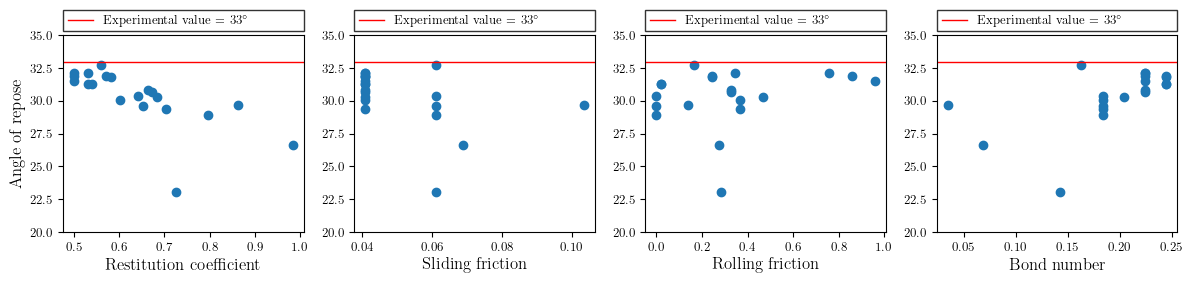
\includegraphics[scale=0.51]{rf_sand.png}
    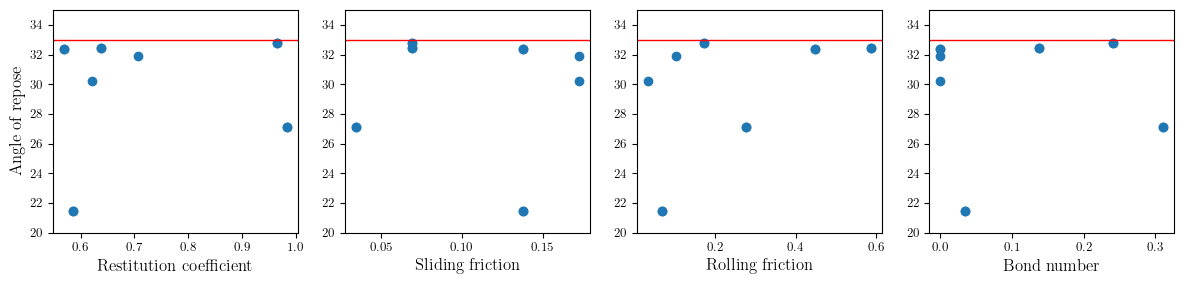
\includegraphics[scale=0.51]{nn_sand.png}
    \caption{\textit{From top to bottom,} valid contact law parameters identified by Random Forest and Neural Network model for quartz sand, and their respective simulation results.}\label{fig:SandNNRF}
\end{figure}

\begin{table}[H]
    \centering
    \resizebox{\textwidth}{!}{%
    \begin{tabular}{cccc|c}
    Restitution coefficient & Sliding friction & Rolling friction & Bond number & Angle of repose \\ \hline
    \textbf{0.5690} & \textbf{0.1379} & \textbf{0.4483} & \textbf{0} & \textbf{32.3822} \\
    0.7069 & 0.1724 & 0.1035 & 0 & 31.9092 \\
    0.6207 & 0.1724 & 0.0345 & 0 & 30.2535 \\
    \textbf{0.6379} & \textbf{0.0690} & \textbf{0.5862} & \textbf{0.1379} & \textbf{32.4170} \\
    0.5862 & 0.1379 & 0.0690 & 0.0345 & 21.4586 \\
    \textbf{0.9655} & \textbf{0.0690} & \textbf{0.1724} & \textbf{0.2414} & \textbf{32.7969} \\
    0.9828 & 0.0345 & 0.2759 & 0.3104 & 27.0953 \\
    0.5862 & 0.1379 & 0.0690 & 0.0345 & 21.4586 \\
    \textbf{0.9655} & \textbf{0.0690} & \textbf{0.1724} & \textbf{0.2414} & \textbf{32.7969} \\
    0.9828 & 0.0345 & 0.2759 & 0.3104 & 27.0953
    \end{tabular}%
    }
    \caption{Valid contact law parameters identified by the NN model for quartz sand and their respective simulation results.}\label{table:sandNN}
\end{table}

\begin{table}[H]
    \centering
    \resizebox{\textwidth}{!}{%
    \begin{tabular}{cccc|c}
    Restitution coefficient & Sliding friction & Rolling friction & Bond number & Angle of repose \\ \hline
    \textbf{0.5612} & \textbf{0.0612} & \textbf{0.1633} & \textbf{0.1633} & \textbf{32.7325} \\
    \textbf{0.5000} & \textbf{0.0408} & \textbf{0.7551} & \textbf{0.2245} & \textbf{32.1187} \\
    0.5000 & 0.0408 & 0.8571 & 0.2245 & 31.8814 \\
    \textbf{0.5306} & \textbf{0.0408} & \textbf{0.3469} & \textbf{0.2245} & \textbf{32.1125} \\
    0.6429 & 0.0612 & 0 & 0.1837 & 30.3771 \\
    0.5714 & 0.0408 & 0.2449 & 0.2449 & 31.8564 \\
    0.6020 & 0.0408 & 0.3674 & 0.1837 & 30.0461 \\
    0.5408 & 0.0408 & 0.0204 & 0.2449 & 31.2764 \\
    0.5000 & 0.0408 & 0.9592 & 0.2245 & 31.5459 \\
    0.5816 & 0.0408 & 0.2449 & 0.2449 & 31.8087 \\
    0.6531 & 0.0612 & 0 & 0.1837 & 29.6271 \\
    0.7041 & 0.0408 & 0.3674 & 0.1837 & 29.3786 \\
    0.6633 & 0.0408 & 0.3265 & 0.2245 & 30.8579 \\
    0.5306 & 0.0408 & 0.0204 & 0.2449 & 31.2787 \\
    0.6735 & 0.0408 & 0.3265 & 0.2245 & 30.6531 \\
    0.7959 & 0.0612 & 0 & 0.1837 & 28.9042 \\
    0.6837 & 0.0408 & 0.4694 & 0.2041 & 30.2650 \\
    0.7245 & 0.0612 & 0.2857 & 0.1429 & 23.0546 \\
    0.8621 & 0.1035 & 0.1379 & 0.0345 & 29.6629 \\
    0.9828 & 0.0690 & 0.2759 & 0.0690 & 26.6594
    \end{tabular}%
    }
    \caption{Valid contact law parameters identified by the RF model for quartz sand and their respective simulation results}
    \label{table:sandlRF}
\end{table}
    
\subsection{Discussion} 

In the current approach, NN and RF models have demonstrated the ability to capture the bulk DPM behavior and generate a database that can then be used to interpolate bulk parameters. Due to limited training data, it is not expected that the models would have a high accuracy in the interpolation step, so a validation step is needed. However, the current number of valid combinations does not meet the expectations of a calibration problem. This can be seen in the quartz sand's RF model: multiple combinations that have been marked as valid by the model have either the same sliding friction or bond number~-~and this is the case for the NN model with limestone as well. One possible solution for this is to extend the `valid' combination range from the current $33\pm0.001$~-~however this will result in a lot more valid combinations and thus only be possible if combined with other bulk tests to reduce the number of verification simulations. Only the combinations that produce satisfactory value in all bulk tests will be verified with DEM simulations. 

Another limitation of the supervised approach is that each trained model only accounts for a single contact law~-~in this case is the linear-spring dashpot model. If the current contact law is not appropriate for describing the granular material, choosing another contact law would require a new model. 


\section{Model comparision}\label{section:discussion}

One of the most vital factors in the calibration process of DPM is computational efficiency since each DEM simulation is very costly in terms of resources (for a static AoR, the simulation time varies from 2 to 24 hours each, and other simulations such as Dynamic AoR, shear cell test are even more expensive). 

The current calibration routine using GL for static AoR costs around 120 to 150 DEM simulations for each attempt(therefore, approximately 300 to 400 DEM simulations, taking into account unfinished attempts), depending on how many iterations are needed. Moreover, most of the time, GL will deliver an adequate solution~-~except the first attempt with limestone, as mentioned in section~\ref{section:GLPerformance}, where GL sampled combinations clusters in the wrong location. Meanwhile, with the current implementation of supervised models, 400 to 500 DEM simulations would be necessary to train the models, and about 20 more are necessary to verify the combinations that supervised models output (training and interpolating time are not taken into account here since they are negligible compare to simulation time). However, from the data obtained, NN and RF models can output more valid combinations than GL. This is crucial since one combination that is valid for this bulk parameter might not work for another bulk parameter, as mentioned in section~\ref{section:Introduction}. 

One major strength of GL and NN is that it has been implemented and tested in several use case (see~\cite{gl-performancestudy,gl-quantification} for GL), while Random Forest models~-~a relatively known algorithm in machine learning, has not been verified against more complex contact laws in the calibration problem to date. 

\section{Conclusion}\label{section:conclusion}
This research has demonstrated three methods of using machine learning to takle the calibration problem of Discrete Particle Model, namely GrainLearning, Neural Network, and Random Forest algorithm within the scope of one bulk parameter, the static angle of repose. Overall, it has been found out that all algorithms have the ability to search for a correct microparameters combinations, to reproduce the exact static AoR in MercuryDPM compare to the experimental value~-~albeit in vastly different ways. While GL iteratively samples the new set of parameter that is getting closer to the optimal value conditioned on previously-learned knowledge, NN and RF models require a two-step method: training with different DEM simulations, then feed it with multiple combinations and select the output that match the experimental values, and verify it using a DEM simulation. It has also shown that GrainLearning has an inconsistent performance 

\pagebreak 



\bibliography{citation}


\end{document}
 